\section{Confidence in communities}\label{confidence-in-communities}

Although it is counterintuitive, completely random graphs, when viewed a
certain way, can be seen to have community structure. In a random graph,
known as an Erdős--Rényi graph \autocite{erdos_evolution_1960}, every
node has an equal probability of being linked to every other node.
Fig.~\ref{fig:randomcommunities} shows how a random graph can show group
structure. The top left shows the adjacency matrix of a random graph
with nodes in arbitrary order; this looks like random white noise. By
rearranging the order of the nodes in the same random graph, as in the
other panes of the figure, a community structure becomes apparent. This
is not actual community structure we are interested in, but rather
artifacts of the randomness. Nevertheless, community detection methods
can pick up on them and find artificial structure in what should be
random. These effects are even more pronounced for sparse graphs, a
category which includes most real-world networks we would like to
analyze \autocite{fortunato_community_2016}.

\begin{figure}
\centering
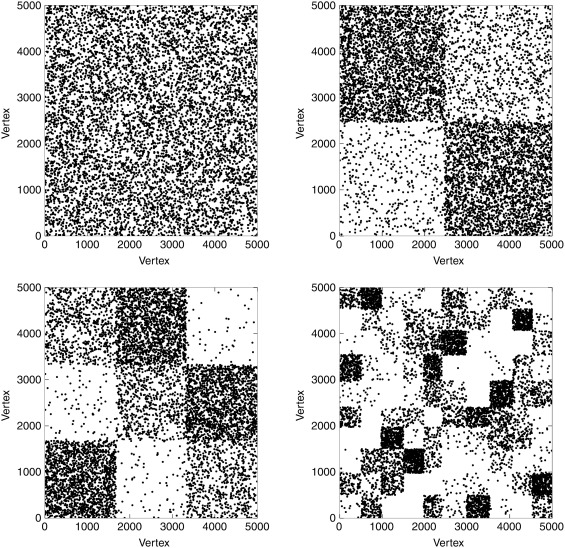
\includegraphics{img/fortunato2016_fig29_randomcommunities.jpg}
\caption{Artificial community structure in a random graph. Each of the
four graphs represent the adjacency matrix of the same 5000-node random
graph, in which every pair of nodes has equal probility of sharing a
link. The top right matrix shows the nodes in arbitrary order, and the
impression is one of random white noise. The others are simply
rearrangements of the nodes for the same random graph. A community
structure can be seen from what is actually random fluctuations in the
network construction process. Figure from
\autocite{fortunato_community_2016}.}\label{fig:randomcommunities}
\end{figure}

section 14 in fortunato 2010:

The first three examples all relate to introducing noise into the edges?
How are they different from each other?

Massen and Doye\ldots{} temperature, thermodynamics. could be in
interesting, but a lot of problems, and rely heavily on modularity---not
clear how it would apply to other quality functions like map equation.

Comparing with a random graph with similar properties:

Bianconi et al. compares entropy of clustering with the average entropy
of an ensemble with the same degree sequence but a random permutation of
the cluster labels.

As fortunato points out: What is unrealistic about the typical null
model is that any node can be connected to any other with equal
probability. Typically large networks have nodes that have some
``horizon'' of other nodes that they can reasonably be expected to be
connected to. ``How to define such ``horizons'' and, more in general,
realistic null models is still an open problem.''

see also fortunato and hric 2016

also\ldots{} latent space models? stochastic block models?

random seed: I think the louvain paper talks about this (blondel)
